%
% ql.tex -- Charakteristiken für quasilinear PDGL 1. Ordnung
%
% (c) 2019 Prof Dr Andreas Müller, Hochschule Rapperswil
%
\documentclass[tikz,12pt]{standalone}
\usepackage{amsmath}
\usepackage{times}
\usepackage{txfonts}
\usepackage{pgfplots}
\usepackage{csvsimple}
\usetikzlibrary{arrows,intersections,math}
\begin{document}
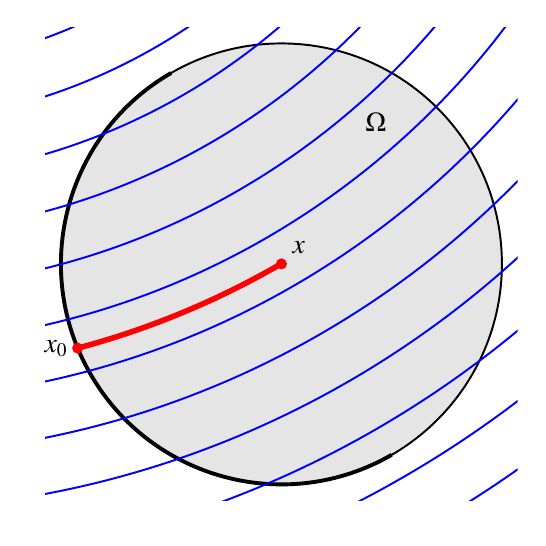
\begin{tikzpicture}[>=latex]

\def\radius{2.8}
\def\l{10.583}

\fill[color=gray!20] (0,0) circle[radius={\radius}];
\draw[line width=0.7pt] (0,0) circle[radius={\radius}];
\draw[line width=1.4pt] ({\radius*cos(120)},{\radius*sin(120)}) arc(120:300:{\radius});

\coordinate (Z) at ({cos(120)*\l},{sin(120)*\l});

\begin{scope}
\clip (-3,-3) rectangle (3,3);
\foreach \R in {1.1,1.8,...,20}{
	\draw[color=blue,line width=0.7pt] (Z) circle[radius={\R}];
}
\end{scope}

\pgfmathparse{90-atan(\radius/(2*\l))}
\xdef\al{\pgfmathresult}

\coordinate (B) at ({\radius*(cos(120+\al))},{\radius*(sin(120+\al))});

\draw[color=red,line width=2pt] (B) arc({2*\al-240}:-60:{\l});
\fill[color=red] (B) circle[radius=2.0pt];
\fill[color=red] (0,0) circle[radius=2.0pt];

\node at (0,0) [above right] {$x$};
\node at (B) [left] {$x_0$};

\node at (1.2,1.8) {$\Omega$};

\end{tikzpicture}
\end{document}

